\section{Our Proposed Approach}\label{sec:approach}
\par In this section, a novel approach of adaptively the Spark configurations platform is proposed, and based on the model; several common machine learning algorithms for configuration parameter tuning are explored. And then the specific details of parameter selection, coding method, evaluation function, weighted allocation, chaos handling, data collection, and training, testing and parameter space searching are described. Finally, the models are evaluated in their accuracy, computational performance, and their sensitivity to various variables such as size of training data, application characteristics.

\par A greedy algorithm is an algorithmic paradigm that follows the problem solving heuristic of making the locally optimal choice at each stage\cite{greedy} with the hope of finding a global optimum. In many problems, a greedy strategy does not in general produce an optimal solution, but nonetheless a greedy heuristic may yield locally optimal solutions that approximate a global optimal solution in a reasonable time. For example: Particle Swarm Optimization Algorithm(PSO), Ant Colony Optimization Algorithms(ACO), Simulated Annealing Algorithm(SA) etc.  PSO is very popular of all, it has a good convergence of the sequence of solutions. However PSO will always get a local optimalization. This means that determining convergence capabilities of different PSO algorithms and parameters therefore still depends on empirical results. So we will attempt at addressing this issue is the development of an "orthogonal learning" strategy for an improved use of the information already existing in the relationship between p and g, so as to form a leading converging exemplar and to be effective with any PSO topology. The aims are to improve the performance of PSO overall, including faster global convergence, higher solution quality, and stronger robustness\cite{PSO2011}.
\par In this paper, we explore to select some key parameters of Spark configureation which will speed up its performance, and compose them to different setting soluations as the particle positions based on PSO algorithm.  We will also introduce  orthogonal learning strategy for improving the PSO performance. Furthermore we will get the global optimalization and improve the performance of Spark.
\par The flowchart of our proposed approach is shown in Fig. \ref{fig:flowchart}.
\begin{figure}\center
	\includegraphics[width=8cm]{flowchart.png}
	\caption{The flowchart of our proposed approach.}\label{fig:flowchart}
\end{figure}
\par From Figure \ref{fig:flowchart}, our approach is described as the following six steps. The parameter is discussed in Section \ref{subsec:parameters}. A coding method of particle positions is presented in Section \ref{subsec:coding}. A object function $f_x()$ for evaluation will be proposed in Section \ref{subsec:evaluation}. The weight factors are given in Section \ref{subsec:weight}. Finally, the construction work of learning examplar detailed in Section \ref{subsec:construct}.
\subsection{Parameters Selection}\label{subsec:parameters}
\par In this work, we will select some key parameters from hundreds of Spark parameters. Specially, we investigate the JVM heap, which is key component of Spark. We can see it from Firgure \ref{fig:ParametersJVM} as follows.
\begin{figure}
	\centering
	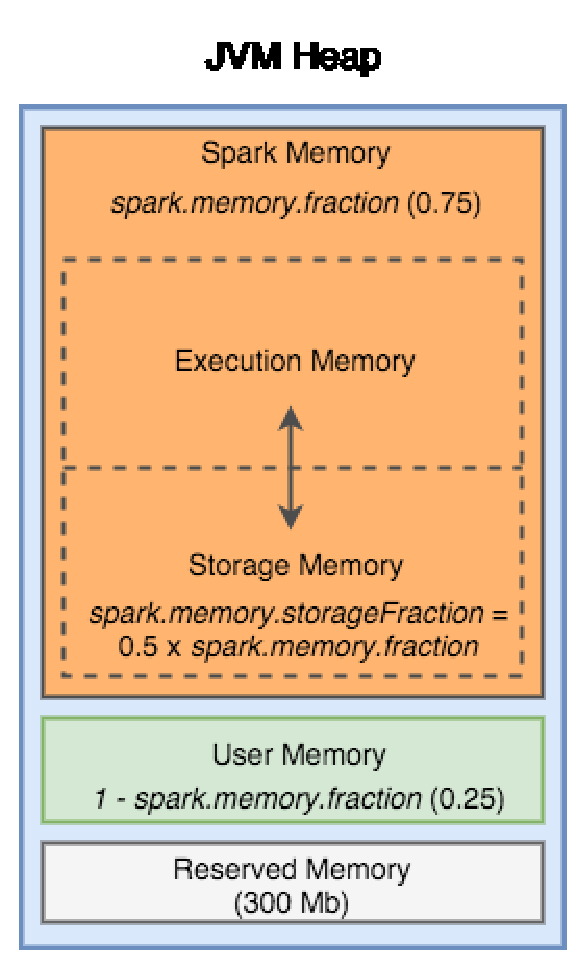
\includegraphics[height=10cm]{3.eps}
	\caption{Parameters of JVM Heap}\label{fig:ParametersJVM}
\end{figure}
 \par Finally, twenty-two parameters are selected, which are shown in Table~\ref{tab:parameters}.  In Table~\ref{tab:parameters}, the ‘Default’ column lists the default value of each parameter. The 'Meaning' column  explains the meaning of this parameter. The ‘rules of thumb’ column lists the values of each parameter that the industry recommends [13][14], and the 'Importance' column is brief introduce the reasons of selection.  The principle for selecting these parameters are listed as follows. 1), the influences of these parameters cover almost all of the available resources in a cluster, such as CPU, Memory, and Disk. 2), these parameters have a great impact on different modules of Spark, such as schedule, shuffle and compress modules. 3), these parameters have impact in different levels of a cluster, such as machine-level, cluster-level. Generally speaking, various factors that affect the performance of the cluster are comprehensively considered. Based on our testing expertise, these parameters that have significant impact on the performance of Spark are selected.

\begin{table*}[t]
\caption{Selected Parameters In Our Approach} \label{tab:parameters} 
\begin{center}
    \begin{tabular}{ | c | c  | p{5cm} | c | p{5cm} |}
    \hline
    Parameter Name & Default & Meaning & Rules of Thumb & Importance\\ 
    \hline
    spark.driver.memory & 512m & Amount of memory to use for the driver process. & 1g-4g & Directly affect computing performace of spark memory.\\ 
    \hline
    spark.driver.maxResultSize & 1g & Each Spark action in the total size of the serialization results for all partitions. & 1g-8g & It represents a fixed memory overhead per reduce task.\\ 
    \hline
    spark.executor.memory &  1g &Amount of memory to use per executor process.   & 2g-8g & Directly affect computing performace of spark memory.\\
    \hline
     spark.driver.cores & 1 & Number of cores to use for the driver process. & 1-8. & Directly affect the parallelism of the program.\\
    \hline
      spark.executor.cores &  1 & Number of cores to use  per executor process. & 10-40 & Directly affect the parallelism of the program.\\
    \hline
     spark.shuffle.file.buffer &  32k & Size of the in-memory buffer for each shuffle file output stream. & 10-40 & These buffers reduce the number of disk seeks and system calls made in creating intermediate shuffle files.\\
    \hline
     spark.reducer.maxSizeInFlight &  48m & Maximum size of map outputs to fetch simultaneously from each reduce task.  & 24k-96k & This represents a fixed memory overhead per reduce task. \\
    \hline
     spark.shuffle.compress &  true & Whether to compress map output files. & true/false & It will speed up the shuffle action.\\
    \hline
     spark.shuffle.spill.compress &  true & Whether to compress data spilled during shuffles. & true/false & It will speed up the shuffle action.\\
    \hline
     spark.broadcast.compress &  true & Whether to compress broadcast variables before sending them. & true/false & It will speed up the broadcast action.\\
    \hline
     spark.io.compression.codec &  lz4 & The codec used to compress internal data such as RDD partitions, event log, broadcast variables and shuffle outputs. & lz4/lzf/snappy. &  It will speed up all of I/O action.\\
    \hline
     spark.rdd.compress &  false & Whether to compress serialized RDD partitions. & true/fasle & It can save substantial space at the cost of some extra CPU time.\\
    \hline
     spark.default.parallelism &  0.6 & Default number of partitions in RDDs returned by transformations. & 0.4-0.8 & It will add RDD parallelism when user operate join, reduceByKey, and parallelize.\\
    \hline
     spark.memory.fraction &  0.6 & Fraction of (heap space - 300MB) used for execution and storage & 0.4-0.8 & The purpose of this config is to set aside memory for internal metadata, user data structures, and imprecise size estimation in the case of sparse, unusually large records. \\
    \hline
     spark.memory.storageFraction &  0.5  & Amount of storage memory immune to eviction, expressed as a fraction of the size of the region set aside by it. & 0.3-0.8 & The higher this is, the less working memory may be available to execution and tasks may spill to disk more often.\\
       \hline
     spark.broadcast.blockSize &  4m & Size of each piece of a block for TorrentBroadcastFactory. & 2m-8m & It will affect parallelism during broadcast.\\
      \hline
    spark.files.useFetchCache &  true & File fetching will use a local cache that is shared by executors that belong to the same application, which can improve task launching performance when running many executors on the same host. & true/false & This optimization may be disabled in order to use Spark local directories that reside on NFS filesystems.\\    
  \hline
     spark.files.openCostInBytes &  4M & The estimated cost to open a file, measured by the number of bytes could be scanned in the same time. & true/false &the partitions with small files will be faster than partitions with bigger files.\\
  \hline
     spark.storage.memoryMapThreshold &  2m & Size of a block above which Spark memory maps when reading a block from disk. & 1m-4m & It prevents Spark from memory mapping very small blocks.\\
  \hline
    spark.rpc.message.maxSize & true & Maximum message size (in MB) to allow in "control plane" communication. & true/false & It will speed up the network action when  you are running jobs with many thousands of map and reduce tasks.\\
  \hline
    spark.speculation.quantile &  0.75 & Fraction of tasks which must be complete before speculation is enabled for a particular stage. & 0.45-0.9 & It will speed up the task.\\
  \hline
     spark.dynamicAllocation.enabled &  true & Whether to use dynamic resource allocation, which scales the number of executors registered with this application up and down based on the workload. & true/false & It will increase the resource when we are handling a workload .\\
   \hline    
    \end{tabular}
\end{center}	
\end{table*}

\par However, parameter selection in a PSO performance model is a non-trivial research issue, which can’t only depend on the domain experts; we will make up on this in the future work.

\subsection{Coding Method}\label{subsec:coding}
\par Type of Spark parameters have some difference type, such as: Float, Interger, Enumeration, Boolean. Because binary coding will occur the mapping errors when it discretize in the continuous function, in this paper we will adopt the floating coding method. The length of coding is decided by num of parameters. We assume a set of parameters as  $A={p_1, p_2, \cdots,  p_N}$, the value of floating coding will be as $V={v_1, v_2, \cdots , v_N}$. It is shown in Table~\ref{tab:coding}  as follows.

\begin{table}[h]
\caption{Coding of Floating Number} \label{tab:coding} 
\begin{center}
    \begin{tabular}{l*{5}{c}r}
    \hline
    Floating Number & $a_1$ & $a_2$ & $a_3$ & $\cdots$ & $a_N$ \\
    \hline
    Coding & $v_1$ & $v_2$ & $v_3$ & $\cdots$ & $v_N$  \\
    \hline
    \end{tabular}
\end{center}
\end{table}
\par Other types of parameters values also need to convert to floating type.  We assume the range of integer and floating values of parameter  are  $(R^{min}, R^{max}) $, and the range of enumeration is $(R_1, R_2, \cdots, R_N)$. Therefore we will get the normalization and anti-normalization formula as follows:
\begin{equation}
R = \left\{ 
\begin{array}{l l l l}
\frac{R-  R^{min} }{ R^{max}-R^{min} } & Float~type \\
\frac{R-  R^{min} }{ R^{max}-R^{min} }  & Interger~type \\
R= true?1.0 : 0.0 & Boolean~type \\
\frac{i}{N} & Enumeration~type, R= R_i  
\end{array} \right.
\end{equation}

\begin{equation}
R = \left\{ 
\begin{array}{l l l l}
R' \times {(R^{max}-R^{min})} +R^{min} & Float\\
round(R' \times (R^{max}-R^{min}) + R^{min})  & Interger\\
round(R')= 1?true : false & Boolean\\
{R_{round(R' \times N)}} & Enum
\end{array} \right.
\end{equation}
\par Using this coding method will guarantee robustness and completeness of coding, But there are always exist multiple solutions of the coding space. Therefore, It does not satify the uniqueness. In this paper, we proposed a new method as follows. After a particle movement, the new position is adjusted. The new position is first normalized to obtain the actual attribute value; then the obtained value is normalized. Since the definition domain and the range of the inverse normalization formula are one-to-one correspondence, the solution of the problem space and the location of the coding space are also one-to-one correspondence. Consequently, it will ensure that the floating coding used satisfy  non-redundancy in this paper.
\subsection{Evaluation Function}\label{subsec:evaluation}
\par As we known, The key criterion of evaluating configuration solution is job time. Therefore, we will choose job time as the evaluation function. We assume that the position $X_{ij}$of particle $ \mathit{i} $ obtained after the $j$th iteration, and  the running time of selected configration is $t(X_{ij})$. So the objective function is expressed as $f=t(X_{ij})$.
\subsection{Weighted Allocation}\label{subsec:weight}
\par The particle swarm optimization algorithm always maintains an acceleration in the case of constant inertia, which facilitates global search at the beginning. However, as the number of iterations increasing, the particles should gradually change from global search to local search. Therefore, the inertia weight should be gradual reduced. Paper [???] proposed a inertia weight method to handle it. The inertia weight $w$ is designed as a linearly reduced function, and the formula is as follows.
\begin{equation}
w=w_{max}-\frac{w_{max}-w_{min}}{iter_{max}} \times k
\end{equation}
where the $ w_{max} $ stands for the initial weight, the $ w_{min} $ stands for the final weight. The general values are 0.9 and 0.4 respectively. and $ iter_{max} $ and $ k $ are the max iterations and the current iterations. After modified the inertia weight, particle will transit from global searching to local searching. It guarantees that the alogithm wil have the good convergence. The speed and position of particle will formula as follows.
\begin{equation}
V^{k+1}_{ij} = wV^{k}_{ij} + C_1 R_1(pbest_{ij}-X^k_{ij}) + C_2 R_2 (gbest_j-X^k_{ij})
\end{equation}
\begin{equation}
X^{k+1}_{ij} = X^{k}_{ij} + V^{k+1}_{ij}
\end{equation}
\subsection{Construct the Learning Examplar}\label{subsec:construct}
\par The orthogonal experimental design (OED) offers an ability to discover the best combination levels for different factors with a reasonably small number of experimental samples [19], [20]. We  use the OED method to construct a promising learning exemplar. OED is used to discover the best combination of a
particle’s best historical position and its neighborhood’s best historical position. The orthogonal experimental factors are the dimensions of the problem and the levels of each dimension (factor) are the two choices of a particle’s best position value and its neighborhood’s best position value on this corresponding dimension.
\par Let $f_m$ denote the experimental result of the $m$th ($1\leq m \leq M$) combination and $S_nq $ denote the effect of the $q$th ($1 \leq q \leq Q$) level in the $n$th ($1 \leq n \leq N$) factor. The calculation of $S_nq$ is to add up all the $f_m$ in which the level is $q$ in the $n$th factor, and then divide the total count of $z_mnq $, as shown in (6) where $z_mnq $ is 1 if the $m$th experimental test is with the $q$th level of the $n$th factor, otherwise, $z_mnq $ is 0.
\begin{equation}
 S_nq = \frac{\sum_{m=1}\nolimits M f_m \times z_mnq}{\sum_{m=1}\nolimits M z_mnq}
\end{equation}
In this way, the effect of each level on each factor can be calculated and compared. Compare $f(i)$ and $f (j)$ and the level combination of the better solution is used to construct the vector. A method to further
reduce the number of the orthogonal combinations is to divide the dimensions into several disjoint groups and regard each group as a factor. This method also may be good for the problems whose dimensions are not independent of each other.




